\documentclass{standalone}
\usepackage{pgfplots}
\pgfplotsset{compat=1.18}
\pgfplotsset{every tick/.append style={color=black}} % applies to major and minor ticks,
\pgfplotsset{every minor tick/.append style={thin}}  % applies only to minor ticks,
\pgfplotsset{every major tick/.append style={thick}} % applies only to major ticks.
\pgfplotsset{every tick label/.append style={font=\tiny}}
\usepackage{amsmath} % for \pi and \frac

\begin{document}
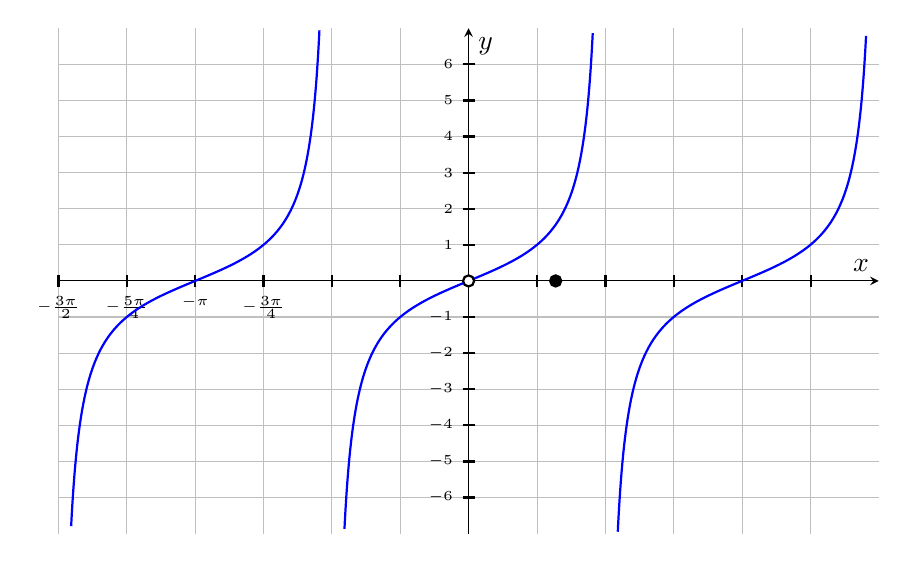
\begin{tikzpicture}
  \begin{axis}[
    height=8cm, width=12cm,
    %domain=-2*pi:2*pi,
    %domain=-5.5:5.5,
    %samples=200,
    axis lines=center,
    xlabel={$x$}, ylabel={$y$},
    %xtick={-2*pi, -3*pi/2, -pi, -pi/2, 0, pi/2, pi, 3*pi/2, 2*pi},
    %xtick={-pi/2, -pi/4, 0, pi/4, pi/2}, %% undelete
    xtick={-3*pi/2,-5*pi/4,...,3*pi/2},
    %xticklabels={$-2\pi$, $-\tfrac{3\pi}{2}$, $-\pi$, $-\tfrac{\pi}{2}$, $0$, $\tfrac{\pi}{2}$, $\pi$, $\tfrac{3\pi}{2}$, $2\pi$},
    xticklabels={$-\tfrac{3\pi}{2}$,$-\tfrac{5\pi}{4}$,$-\pi$,$-\tfrac{3\pi}{4}$},
    %xticklabels={$-\tfrac{\pi}{2}$, $-\tfrac{\pi}{4}$, $0$, $\tfrac{\pi}{4}$, $\tfrac{\pi}{2}$},
    ytick={-6,...,6},%{,-8,...,10}
    restrict y to domain=-7:7,
    xmin=-1.5*pi, xmax=1.5*pi,
    ymin=-7, ymax=7,
    grid=both,
    enlargelimits=false,
    clip=false
  ]
    \addplot[samples=2000,domain=-1.5*pi:1.5*pi, color=blue, thick]{tan(deg(x))};
    %\addplot[red, thick, domain=0:1, samples=1000] {x+1};
    %\addplot[purple, thick, domain=-1.5:-0.5, samples=1000] {3*(x-1)^2-4};
    
    % endpoints
    \filldraw[color=black, fill=white, thick](0,0) circle (2pt);
    \filldraw[black, thick](1,0) circle (2pt);
  \end{axis}
\end{tikzpicture}
\end{document}
